\subsection{Linear Classifiers}
\label{sub:linear_classifiers}
On a un input qui est transformé en vecteur de features et finalement on aura un résultat.
\begin{example}
    Voici un exemple de classification linéaire :
    \begin{itemize}[label=\textbullet]
        \item input : un mail
        \item feature : le nom, le nombre de fautes d'ortographes, ...
        \item résultat : spam ou non
    \end{itemize}
\end{example}

Dans les classifieurs linéaires, l'input sont les features où chaque feature a un poids. L'activation est la somme des produits
des features et des poids :
\begin{equation*}
    \text{activation}_w(x) = \sum_{i=1}^{n} w_i\cdot f_i(x) = w\cdot f(x)
\end{equation*}
Si l'activation est \textbf{positive}, l'output sera égal à +1 sinon -1. 

\subsection{Weights}
\label{sub:weights}
Pas très bien compris cette partie mais en soit on fait le produit des vecteurs de poids :
\begin{figure}[H]
    \centering
    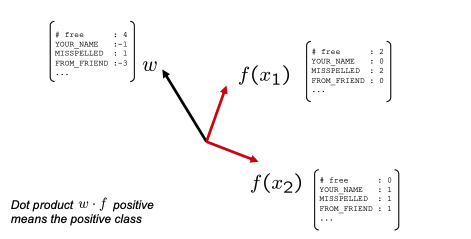
\includegraphics[scale=0.6]{pictures/weights_product.png}
    \caption{Produit des vecteurs de poids}
\end{figure}


\subsection{Binary Decision Rule}
\label{sub:binary_decision_rule}
Dans l'espace des vecteurs de features, les exemples sont des points et chaque vecteur de poids est un hyperplan, où un côté
correspond à +1 et l'autre à -1.
\begin{example}
    Pour $w$, on a les features suivants : $\texttt{free} : 4$, $\texttt{money} : 2$. On a $f \cdot w > 0$ quand $4\cdot f_{free} + 2\cdot f_{money} > 0$.
    L'inverse pour $<0$. Ces équations correspondent aux deux moitiés de l'hyperplan.
\end{example}

\subsection{Weights Updates}
\label{sub:weights_updates}
On commence avec tous les poids égaux à 0. Pour chaque instance d'entrainement :
\begin{itemize}[label=\textbullet]
    \item On classifie les poids actuels.
    \item Si c'est \textbf{correct}, on ne change pas.
    \item Si c'est \textbf{incorrect}, on ajuste le vecteur de poids.
\end{itemize}

\begin{example}
    Voyons sur un exemple :
    \begin{figure}[H]
        \centering
        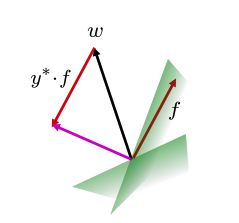
\includegraphics[scale=0.6]{pictures/example_waights_update.png}
        \caption{Exemple de mise à jour des poids}
    \end{figure}
    Ici, pour classifier les poids actuels, on utilise :
    \begin{equation*}
        y=
        \begin{cases}
            +1 & \text{si } w\cdot f(x) > 0\\
            -1 & \text{si } w\cdot f(x) < 0
        \end{cases}
    \end{equation*}
    Si c'est correct, comme dit, on ne change rien. Par contre si ce n'est pas le cas, on ajuste le vecteur de poids en ajoutant
    ou en enlevant le poids du vecteur. On a donc :
    \begin{equation*}
        w = w+y^*\cdot f
    \end{equation*}
    On calcule : 
    \begin{equation*}
        w' \cdot f = (w+y^*\cdot f)\cdot f = w\cdot f + y^*\cdot f\cdot f
    \end{equation*}
\end{example}

\subsection{Multiclass Decision Rule}
\label{sub:multiclass_decision_rule}
C'est assez rare d'avoir une distinction binaire, on a souvent plus de deux classes. Ici, c'est plus intéressant d'avoir 
un vecteur de poids par classe $w_y$. Pour une classe $y$ on a le score (activation) $w_y\cdot f(x)$. Les meilleures prédictions
sont celles avec le meilleur score $y=\text{argmax}_{y} w_{y}\cdot f(x)$.
\begin{figure}[H]
    \centering
    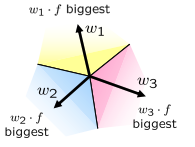
\includegraphics[scale=0.6]{pictures/multiclass_perceptron.png}
    \caption{Exemple de multiclass decision rule}
\end{figure}
\begin{example}
    On peut garder à peu près la même règle, commençons avec tous les poids à 0. Avec les poids actuels :
    \begin{equation*}
        y = \text{argmax}_{y} w_{y}\cdot f(x)
    \end{equation*}
    Si c'est correct, on ne change pas. Si par contre ce n'est pas correct, on fait :
    \begin{equation*}
        w_y = w_y - f(x)
    \end{equation*}
    et
    \begin{equation*}
        w_{y^*} = w_{y^*} + f(x)
    \end{equation*}
    \begin{figure}[H]
        \centering
        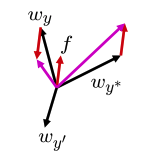
\includegraphics[scale=0.6]{pictures/mutliclass_example.png}
        \caption{Exemple de multiclass decision rule}
    \end{figure}
\end{example}

\subsection{Propriétés des Perceptrons}
\label{sub:propriétés_des_perceptrons}
\begin{itemize}
    \item \textbf{Séparabilité} : Si les données sont séparées parfaitement.
    \item \textbf{Convergence} : Si les données sont séparables, le perceptron peut converger.
    \item \textbf{Mistake Bound} : Le nombre maximal d'erreurs de la marge/degré de séparabilité.
\end{itemize}


\subsection{Problèmes des Perceptrons}
\label{sub:problèmes_des_perceptrons}
\begin{itemize}
    \item \textbf{Noise} : Si les données ne sont pas séparables les poids peuvent diverger.
    \item \textbf{Mauvaise généralisation} : Trouve une solution partielle qui ne généralise pas bien.
    \item \textbf{Overtraining} : La précision augmente et puis diminue, donc il faut arrêter d'apprendre avant que la 
    précision diminue.
\end{itemize}

\subsection{Améliorations des Perceptrons}
\label{sub:améliorations_des_perceptrons}
\begin{figure}[H]
    \centering
    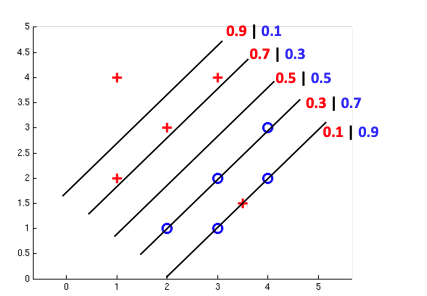
\includegraphics[scale=0.6]{pictures/better_perceptrons.png}
    \caption{Améliorations des perceptrons}
\end{figure}
Ici, on n'exclue pas la possibilité qu'il y ait une erreur de classification. On dit qu'il peut y avoir un rouge dans le 
bleu avec une probabilité de 0.1.\\
Comment trouver une décision déterministe ?\\
Le score d'un perceptron est : $z = w\cdot f(x)$. Si $z$ est positif, on veut une probabilité qui va vers 1 et 0 sinon.
Dès lors on a la fonction sigmoïde :
\begin{equation*}
    \phi(z) = \frac{1}{1+e^{-z}}
\end{equation*}
\begin{figure}[H]
    \centering
    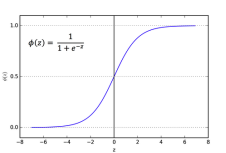
\includegraphics[scale=0.6]{pictures/sigmoid.png}
    \caption{Fonction sigmoïde}
\end{figure}


\subsection{Logistic Regression}
\label{sub:logistic_regression}
On veut maximiser la probabilité d'avoir la bonne classe (likelihood):
\begin{equation*}
    \max_w ll(w) = \max_w \sum_{i=1}^{n} \log P(y_i|x_i;w)
\end{equation*}
Avec :
\begin{equation*}
    \begin{aligned}
        &P(y_i = +1|x_i;w) = \frac{1}{1+e^{-w\cdot f(x_i)}}\\
        &P(y_i = -1|x_i;w) = 1 - \frac{1}{1+e^{-w\cdot f(x_i)}}
    \end{aligned}
\end{equation*}


\subsection{Multiclass Logistic Regression}
\label{sub:multiclass_logistic_regression}
Avec $z_1,z_2$ et $z_3$ les scores des trois classes, on veut les rendre probabilistique :
\begin{equation*}
    z_1,z_2,z_3 \rightarrow \frac{e^{z_1}}{e^{z_1}+e^{z_2}+e^{z_3}}, \frac{e^{z_2}}{e^{z_1}+e^{z_2}+e^{z_3}}, \frac{e^{z_3}}{e^{z_1}+e^{z_2}+e^{z_3}}
\end{equation*}

Pour trouver le meilleur $w$, on cherche le maximum de likelihood :
\begin{equation*}
    \max_w ll(w) = \max_w \sum_{i=1}^{n} \log P(y_i|x_i;w)
\end{equation*}
Avec :
\begin{equation*}
    P(y_i|x_i;w) = \frac{e^{w_{y_i}\cdot f(x_i)}}{\sum_{y} e^{w_{y}\cdot f(x_i)}}
\end{equation*}